%% Relatório AM v3 — Template IEEE (bare_conf)
%% Compilar com pdfLaTeX no Overleaf
%% Upload também a pasta docs/imagens/ (PNG + PDF das 3 figuras) para o projeto Overleaf.

\documentclass[conference]{IEEEtran}

\usepackage[utf8]{inputenc}
\usepackage[T1]{fontenc}
\usepackage[brazil]{babel}
\usepackage{graphicx}
\graphicspath{{imagens/}}
\usepackage{xcolor}
\usepackage{amsmath}
\usepackage{booktabs}
\usepackage{array}
\usepackage{cite}
\usepackage{url}

\renewcommand{\refname}{Referências}
\newcommand{\code}[1]{\texttt{#1}}

\hyphenation{op-tical net-works semi-conduc-tor in-a-dim-plên-cia}

\begin{document}

\title{Aprendizado de Máquina e Ciência de Dados\\
Sistema Híbrido de Credit Scoring para Pequenos Varejistas Utilizando Machine Learning: Um Estudo de Caso na Praso}

\author{\IEEEauthorblockN{1\textsuperscript{st} Discente A}
\IEEEauthorblockA{\textit{Centro de Informática - UFPE} \\
Recife, Brazil \\
discentea@cin.ufpe.br}
\and
\IEEEauthorblockN{2\textsuperscript{nd} Discente B}
\IEEEauthorblockA{\textit{Centro de Informática - UFPE} \\
Recife, Brazil \\
discenteb@cin.ufpe.br}
\and
\IEEEauthorblockN{3\textsuperscript{rd} Discente C}
\IEEEauthorblockA{\textit{Centro de Informática - UFPE} \\
Recife, Brazil \\
discentec@cin.ufpe.br}
\and
\IEEEauthorblockN{4\textsuperscript{th} Discente D}
\IEEEauthorblockA{\textit{Centro de Informática - UFPE} \\
Recife, Brazil \\
discented@cin.ufpe.br}
}

\maketitle

\begin{abstract}
A concessão de crédito para pequenos varejistas representa um desafio devido à escassez de informações financeiras estruturadas e ao risco de inadimplência. A Praso, startup brasileira especializada em distribuição para pequenos estabelecimentos comerciais, utiliza um sistema de análise de crédito baseado em dados cadastrais, informações de bureaus de crédito e dados comportamentais dos clientes. Este trabalho propõe modelos de Machine Learning para previsão de inadimplência utilizando dados de aproximadamente 3.000 clientes, complementados por um sistema híbrido de roteamento que direciona cada cliente ao modelo mais adequado (comportamental, de aplicação ou revisão manual). O modelo comportamental final utiliza 18 \textit{features} derivadas do histórico transacional. Os resultados alcançam ROC-AUC de 0,850 no sistema integrado (ganho de +4,56 pontos percentuais sobre o baseline de aplicação isolado, AUC 0,804).
\end{abstract}

\IEEEpeerreviewmaketitle

\section{Introdução}

\IEEEPARstart{O}{} acesso ao crédito é um dos principais fatores que influenciam a sustentabilidade financeira de pequenos varejistas. Entretanto, a concessão de crédito envolve riscos associados à possibilidade de inadimplência dos clientes, exigindo mecanismos eficientes de avaliação de risco.

A Praso atua no segmento de distribuição para pequenos estabelecimentos comerciais e oferece crédito para seus clientes realizarem compras por meio da plataforma, utilizando informações públicas, dados de crédito e histórico de relacionamento para estimar a probabilidade de inadimplência.

Uma das principais dores do pequeno varejista é o \textbf{ciclo de caixa} --- o tempo médio que a empresa leva para transformar gastos em receita, calculado como $(\mathrm{PME} + \mathrm{PMR}) - \mathrm{PMP}$. No mercado tradicional, fornecedores levam de 2 a 14 dias para avaliar o crédito antes de conceder prazo de pagamento. A Praso se diferencia ao oferecer \textbf{análise de crédito instantânea no momento do cadastro}, desburocratizando o acesso ao crédito.

A utilização de técnicas de Machine Learning permite automatizar esse processo, reduzindo o tempo de análise e melhorando a qualidade das decisões de crédito. O objetivo deste trabalho é desenvolver e avaliar modelos de classificação capazes de prever a probabilidade de inadimplência, integrando informações cadastrais e comportamentais por um sistema de roteamento em três \textit{tiers}.

\section{Análise de Dados e Feature Engineering}

\subsection{Análise Exploratória dos Dados}

O conjunto de dados é composto por duas bases: clientes (informações cadastrais) e pedidos (informações transacionais). A base de clientes possui 3.000 registros com variáveis como segmento, CNAE, capital social, idade do CNPJ, indicadores Serasa e presença digital. A variável alvo é \code{inadimplente}. Foi verificada a unicidade de \code{id\_cliente} e \code{id\_pedido}, sem duplicatas encontradas.

\subsubsection{Análise Exploratória Estrutural}

As variáveis foram classificadas em categóricas (\code{uf}, \code{municipio}, \code{segmento\_cliente}, \code{cnae\_codigo}, entre outras), numéricas (\code{capital\_social}, \code{idade\_cnpj}, indicadores Serasa) e binárias (\code{serasa\_socio\_tem\_negativacao}, \code{inadimplente}).

\textbf{31,3\%} dos clientes possuem histórico de inadimplência e \textbf{68,7\%} são adimplentes (Fig.~\ref{fig:dist-inadimplencia}). Apenas \textbf{664 clientes (22,1\%)} possuem histórico de pedidos (Fig.~\ref{fig:dist-comportamental}); entre eles, a taxa de inadimplência é de \textbf{20,8\%}. Adotamos AUC-ROC, F1 e estratificação como resposta ao desbalanceamento moderado.

\begin{figure}[!t]
    \centering
    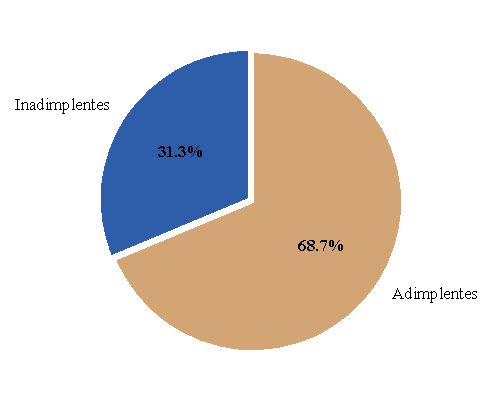
\includegraphics[width=0.95\linewidth]{distribuicao_inadimplencia.pdf}
    \caption{Distribuição de clientes por histórico de inadimplência ($n=3.000$).}
    \label{fig:dist-inadimplencia}
\end{figure}

\begin{figure}[!t]
    \centering
    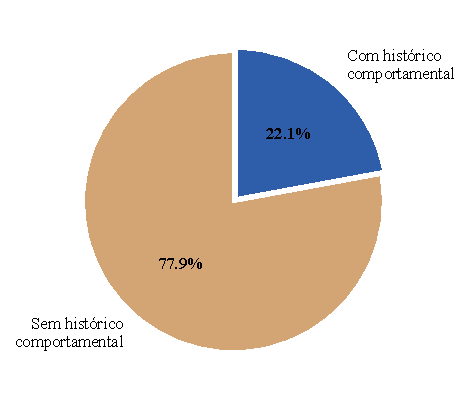
\includegraphics[width=0.95\linewidth]{distribuicao_historico_comportamental.pdf}
    \caption{Distribuição de clientes com e sem histórico comportamental de pedidos.}
    \label{fig:dist-comportamental}
\end{figure}

\subsubsection{Análise de Valores Faltantes e \textit{Outliers}}

Valores faltantes concentram-se em variáveis do iFood e Google Maps (87,9\% a 98,9\%), indicando ausência de presença digital e não erro de coleta. Foram identificados \textit{outliers} em \code{serasa\_contagem\_negativacoes} (máx.\ = 141) e \code{serasa\_contagem\_protestos} (máx.\ = 79), mantidos por representarem alto risco real.

\subsubsection{Análise Univariada}
\label{subsec:analise-univariada}

\code{idade\_cnpj}, indicadores Serasa e presença digital (\code{has\_ifood}, \code{has\_google\_maps}) apresentaram relação relevante com inadimplência.

\subsubsection{Análise Bivariada}

Correlação positiva entre negativações e inadimplência; idade do CNPJ correlaciona negativamente com risco. Padrões confirmados:
\begin{enumerate}
    \item Empresas com mais de 2.400 dias ($\sim$6,5 anos) apresentam menor inadimplência.
    \item \code{serasa\_socio\_tem\_negativacao} associa-se a risco superior.
    \item Protestos (mediana = 0; máx.\ = 79) diferenciam grupos de risco.
    \item Presença no iFood (6,2\%) e Google Maps (1,1\%) associa-se a menor inadimplência.
\end{enumerate}

\subsubsection{Análise Multivariada}

Clientes com histórico comportamental apresentam taxa de 20,8\% de inadimplência, contra 31,3\% na carteira e 33,9\% entre clientes sem pedidos (Fig.~\ref{fig:taxa-grupo}).

\begin{figure}[!t]
    \centering
    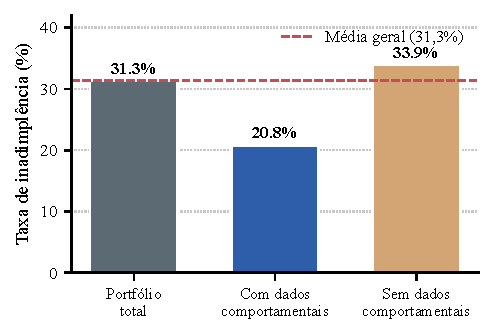
\includegraphics[width=\linewidth]{taxa_inadimplencia_por_grupo.pdf}
    \caption{Taxa de inadimplência por grupo: portfólio total, com e sem dados comportamentais. A linha tracejada indica a média geral (31,3\%).}
    \label{fig:taxa-grupo}
\end{figure}

\subsection{Pré-processamento dos Dados}

\subsubsection{Tratamento de Valores Faltantes}

Foram criadas flags \code{has\_ifood} e \code{has\_google\_maps}. Demais colunas numéricas receberam imputação por mediana. Colunas 100\% nulas (\code{ifood\_contagem\_avaliacoes}, \code{google\_maps\_contagem\_avaliacoes}) foram excluídas.

\subsubsection{Tratamento de \textit{Outliers}}

\textit{Outliers} cadastrais foram mantidos. Para valores de pedidos agregados, aplicou-se \code{log1p} (\code{log\_valor\_mean}, \code{log\_valor\_max}, etc.).

\subsubsection{Detecção e Tratamento de Duplicadas}

Zero duplicatas em \code{id\_cliente} e \code{id\_pedido}.

\subsubsection{Feature Scaling}

\code{StandardScaler} para modelos sensíveis à escala (Regressão Logística). Árvores não exigem escalonamento obrigatório.

\subsubsection{Encoding de Variáveis Categóricas}

\code{segmento\_cliente}, \code{natureza\_juridica} e \code{fonte\_cliente} via \code{pd.get\_dummies}. \code{ifood\_faixa\_preco} e \code{cnae\_divisao} via \code{OneHotEncoder}. CNAE decomposto em divisão (39 valores); Target Encoding e níveis grupo/classe não foram aplicados.

\subsection{Divisão dos Dados}

Divisão \textbf{70\% treino / 30\% teste} estratificada (2.100/900 no Modelo de Aplicação; 464/200 no Comportamental). Hiperparâmetros via \textbf{RandomizedSearchCV} com 3 folds e ROC-AUC (15 iterações na Aplicação; 20 no Comportamental).

\subsection{Feature Engineering}

Intervalos convertidos em pontos médios (\code{capital\_social\_mid}, \code{idade\_cnpj\_mid}, \code{google\_maps\_avaliacao\_mid}). \code{serasa\_credores} $\rightarrow$ \code{serasa\_n\_setores}; criada \code{has\_serasa\_negativacao}.

O modelo comportamental utiliza \textbf{18 \textit{features}}: métricas de valor (\code{valor\_mean}, \code{valor\_max}, etc.), atraso (\code{delay\_mean}, \code{pct\_orders\_delayed}, \code{delay\_spike\_ratio}), frequência (\code{orders\_count}, \code{orders\_per\_month}, \code{recency\_days}) e versões log-transformadas.

\section{Modelagem}

Foram avaliados Regressão Logística, Random Forest e XGBoost, treinados separadamente para o Modelo de Aplicação (3.000 clientes) e Comportamental (664 clientes).

\subsection{Modelo A --- Regressão Logística}

\subsubsection{Conceitos Básicos}
Modelo estatístico para classificação binária que estima probabilidade de inadimplência por combinação linear dos atributos.

\subsubsection{Justificativa}
Baseline interpretável, amplamente utilizado em credit scoring, com \code{class\_weight='balanced'}.

\subsubsection{Espaço de Busca}
\code{C}, \code{penalty} e \code{solver}.

\subsubsection{Hiperparâmetros Selecionados}
\code{class\_weight='balanced'}, \code{max\_iter=1000}, sem tunagem extensiva.

\subsection{Modelo B --- Random Forest}

\subsubsection{Conceitos Básicos}
Ensemble de árvores de decisão com amostragem \textit{bootstrap} e subconjunto de atributos.

\subsubsection{Justificativa}
Captura relações não lineares, robusto a \textit{outliers} e fornece importância de atributos.

\subsubsection{Espaço de Busca}
\code{n\_estimators}, \code{max\_depth}, \code{min\_samples\_leaf}, \code{max\_features}.

\subsubsection{Hiperparâmetros Selecionados}
Melhor modelo Comportamental (RandomizedSearchCV, 3 folds, ROC-AUC): \code{n\_estimators=100}, \code{min\_samples\_leaf=2}, \code{max\_features=log2}, \code{max\_depth=None} (CV ROC-AUC = 0,7484).

\subsection{Modelo C --- XGBoost}

\subsubsection{Conceitos Básicos}
Gradient Boosting com árvores sequenciais corrigindo erros anteriores.

\subsubsection{Justificativa}
Alto desempenho em dados tabulares heterogêneos.

\subsubsection{Espaço de Busca}
\code{n\_estimators}, \code{learning\_rate}, \code{max\_depth}, \code{subsample}, \code{colsample\_bytree}.

\subsubsection{Hiperparâmetros Selecionados}
Melhor modelo Aplicação (RandomizedSearchCV, 3 folds, ROC-AUC): \code{subsample=0,7}, \code{n\_estimators=100}, \code{max\_depth=3}, \code{learning\_rate=0,05}, \code{colsample\_bytree=0,8} (teste ROC-AUC = 0,772).

\subsection{Sistema de Roteamento}

O sistema classifica clientes em três \textit{tiers} com base em dois \textit{scores}:
\begin{itemize}
    \item \textbf{Score A} (riqueza de dados): 0 para clientes sem pedidos; 0,5--1,0 escalonado por \code{orders\_per\_month}.
    \item \textbf{Score B} (complexidade do perfil): maior incerteza do Modelo de Aplicação para $p \approx 0{,}5$.
\end{itemize}
Thresholds: \code{threshold\_A=0,50} e \code{threshold\_B=0,60}. Foi treinado ML Router (Decision Tree) com \code{[score\_A, score\_B, orders\_per\_month, pct\_orders\_delayed, delay\_mean, p\_app]}.

\begin{table}[!t]
\caption{Distribuição de clientes por \textit{tier}}
\label{tab:tiers}
\centering
\small
\begin{tabular}{lllc}
\toprule
\textbf{Tier} & \textbf{Condição} & \textbf{Modelo} & \textbf{Qtd} \\
\midrule
BEHAVIORAL & Score\_A $\geq$ 0,50 & Comportamental & 664 (22,1\%) \\
APPLICATION & Score\_A $<$ 0,50, Score\_B $<$ 0,60 & Aplicação & 998 (33,2\%) \\
MANUAL\_REVIEW & Score\_A $<$ 0,50, Score\_B $\geq$ 0,60 & Revisão humana & 1.338 (44,6\%) \\
\bottomrule
\end{tabular}
\end{table}

\subsection{Tratamento de Desbalanceamento}

SMOTE e undersampling \textbf{não foram aplicados}. Alternativas: \code{class\_weight='balanced'}, estratificação, otimização por ROC-AUC e \textit{thresholds} por \textit{tier}.

\section{Análise e Comparação de Resultados}

A métrica principal foi \textbf{ROC-AUC}, adequada para ranqueamento de clientes por risco.

\begin{table}[!t]
\caption{Modelo de Aplicação --- teste ($n=900$)}
\label{tab:app}
\centering
\small
\begin{tabular}{lccccc}
\toprule
\textbf{Modelo} & \textbf{AUC} & \textbf{Acc.} & \textbf{Prec.} & \textbf{Rec.} & \textbf{F1} \\
\midrule
Logistic Regression & 0,749 & 0,684 & 0,497 & 0,667 & 0,570 \\
Random Forest & 0,738 & 0,723 & 0,579 & 0,429 & 0,493 \\
XGBoost & 0,733 & 0,704 & 0,528 & 0,543 & 0,535 \\
\textbf{XGBoost Tuned} & \textbf{0,772} & \textbf{0,701} & \textbf{0,517} & \textbf{0,723} & \textbf{0,603} \\
\bottomrule
\end{tabular}
\end{table}

\begin{table}[!t]
\caption{Modelo Comportamental --- teste ($n=200$)}
\label{tab:behav}
\centering
\small
\begin{tabular}{lccccc}
\toprule
\textbf{Modelo} & \textbf{AUC} & \textbf{Acc.} & \textbf{Prec.} & \textbf{Rec.} & \textbf{F1} \\
\midrule
Baseline (App-only) & 0,623 & 0,620 & 0,270 & 0,476 & 0,345 \\
Logistic Regression & 0,733 & 0,695 & 0,383 & 0,738 & 0,504 \\
XGBoost & 0,760 & 0,790 & 0,500 & 0,476 & 0,488 \\
Random Forest & 0,775 & 0,795 & 0,556 & 0,119 & 0,196 \\
\textbf{RF Tuned} & \textbf{0,770} & \textbf{0,795} & \textbf{0,514} & \textbf{0,429} & \textbf{0,468} \\
\bottomrule
\end{tabular}
\end{table}

O RF Tuned supera o baseline app-only em \textbf{+14,67 pp} de AUC. O router rule-based alcança ROC-AUC \textbf{0,850} no sistema (3.000 clientes), +4,56 pp sobre baseline (0,804); ML Router: 0,848.

\begin{table}[!t]
\caption{Sistemas de roteamento ($n=3.000$)}
\label{tab:router}
\centering
\small
\begin{tabular}{lcc}
\toprule
\textbf{Sistema} & \textbf{ROC-AUC} & \textbf{$\Delta$} \\
\midrule
Baseline (só Aplicação) & 0,804 & --- \\
\textbf{Router Rule-based} & \textbf{0,850} & \textbf{+4,56 pp} \\
ML Router & 0,848 & +4,32 pp \\
\bottomrule
\end{tabular}
\end{table}

Tempo de inferência não foi medido sistematicamente; espera-se latência $<$10\,ms por cliente.

\section{Interpretabilidade dos Modelos}

Análise via SHAP (TreeExplainer) e \code{feature\_importances\_}. Tabela~\ref{tab:shap-app} resume o modelo de aplicação; Tabela~\ref{tab:shap-behav}, o comportamental.

\begin{table*}[!t]
\caption{Top 10 \textit{features} SHAP --- Modelo de Aplicação (XGBoost Tuned)}
\label{tab:shap-app}
\centering
\small
\begin{tabular}{clcl}
\toprule
\textbf{Rank} & \textbf{Feature} & \textbf{|SHAP|} & \textbf{Direção esperada} \\
\midrule
1 & idade\_cnpj\_mid & 0,553 & Empresas mais novas $\rightarrow$ maior risco \\
2 & serasa\_socio\_tem\_negativacao & 0,370 & Sócio negativado $\rightarrow$ maior risco \\
3 & serasa\_n\_setores & 0,193 & Mais setores $\rightarrow$ maior risco \\
4 & segmento\_cliente (Seg. 16) & 0,141 & Variação setorial \\
5 & fonte\_cliente (Fonte 5) & 0,138 & Canal de aquisição \\
6 & capital\_social\_mid & 0,102 & Proxy de solidez \\
7 & natureza\_juridica (EI) & 0,091 & Forma jurídica \\
8 & serasa\_contagem\_negativacoes & 0,050 & Mais negativações \\
9 & has\_google\_maps & 0,011 & Presença digital \\
10 & serasa\_contagem\_protestos & 0,004 & Protestos \\
\bottomrule
\end{tabular}
\end{table*}

\begin{table*}[!t]
\caption{Top 10 \textit{features} SHAP --- Modelo Comportamental (RF Tuned)}
\label{tab:shap-behav}
\centering
\small
\begin{tabular}{clcll}
\toprule
\textbf{Rank} & \textbf{Feature} & \textbf{|SHAP|} & \textbf{Tipo} & \textbf{Direção} \\
\midrule
1 & idade\_cnpj\_mid & 0,038 & Aplicação & Empresas novas $\rightarrow$ risco \\
2 & delay\_mean & 0,037 & Comportam. & Maior atraso $\rightarrow$ risco \\
3 & orders\_per\_month & 0,037 & Comportam. & Frequência \\
4 & delay\_max & 0,033 & Comportam. & Picos de atraso \\
5 & pct\_orders\_delayed & 0,026 & Comportam. & \% atrasos \\
6 & delay\_spike\_ratio & 0,026 & Comportam. & Picos relativos \\
7 & recency\_days & 0,026 & Comportam. & Recência \\
8 & capital\_social\_mid & 0,013 & Aplicação & Solidez \\
9 & serasa\_socio\_tem\_negativacao & 0,012 & Aplicação & Sócio negativado \\
10 & valor\_mean & 0,009 & Comportam. & Valor dos pedidos \\
\bottomrule
\end{tabular}
\end{table*}

\textit{Features} de atraso dominam o modelo comportamental; idade do CNPJ e Serasa dominam o de aplicação.

\section{Política de Crédito}

A escolha do \textit{threshold} equilibra risco e volume de aquisição. Tabela~\ref{tab:policy-thresh} apresenta \textit{thresholds} por \textit{tier}; Tabela~\ref{tab:policy-scen}, cenários simulados.

\begin{table}[!t]
\caption{\textit{Thresholds} sugeridos por \textit{tier}}
\label{tab:policy-thresh}
\centering
\small
\begin{tabular}{lccc}
\toprule
\textbf{Tier} & \textbf{Aprovar} & \textbf{Manual} & \textbf{Negar} \\
\midrule
BEHAVIORAL & $p < 0{,}25$ & $0{,}25$--$0{,}35$ & $p \geq 0{,}35$ \\
APPLICATION & $p < 0{,}15$ & $0{,}15$--$0{,}25$ & $p \geq 0{,}25$ \\
MANUAL\_REVIEW & --- & $p < 0{,}40$ & $p \geq 0{,}40$ \\
\bottomrule
\end{tabular}
\end{table}

\begin{table}[!t]
\caption{Cenários de política de crédito}
\label{tab:policy-scen}
\centering
\small
\begin{tabular}{lccc}
\toprule
\textbf{Cenário} & \textbf{Aprov.} & \textbf{Auto-Aprov.} & \textbf{Inad.} \\
\midrule
Baseline (App) & 21,4\% & 21,4\% & 5,6\% \\
Router Recomendado & 39,0\% & 25,5\% & 7,3\% \\
Router Restritivo & 21,4\% & 8,2\% & 2,8\% \\
Router Permissivo & 60,7\% & 51,9\% & 11,7\% \\
\bottomrule
\end{tabular}
\end{table}

Casos especiais: limite reduzido para empresas novas; override para sócios negativados ($p < 0{,}10$); redução de limite para \code{pct\_orders\_delayed} $> 0{,}5$.

\section{Conclusão e Discussão}

Este trabalho apresentou um sistema híbrido de credit scoring para a Praso. Principais achados: XGBoost Tuned (AUC 0,772) para aplicação; RF Tuned (AUC 0,770) para comportamental; sistema integrado (AUC 0,850).

\textbf{Limitações:} cobertura comportamental de 22,1\%; 44,6\% em revisão manual; SMOTE não implementado; tempo de inferência não medido; Target Encoding e \textit{features} de interação pendentes.

\textbf{Implicações práticas:} o sistema automatiza a decisão de crédito para $\sim$55\% dos clientes (\textit{tiers} BEHAVIORAL e APPLICATION), mantendo revisão humana para perfis de alta incerteza.

\textbf{Trabalhos futuros:} reamostragem, novas fontes (Receita Federal, Open Banking), calibração de probabilidades, reject inference e survival analysis.

\noindent\textit{Métricas rastreáveis:} \code{models/04\_application\_metrics\_*.json}, \code{models/05\_behavioral\_metrics\_*.json}, \code{models/06\_router\_metrics\_*.json}, \code{data/08\_shap\_importance\_*.csv}, \code{data/09\_credit\_policy\_*.json}.

\begin{thebibliography}{1}

\bibitem{chen2016}
T.~Chen and C.~Guestrin, ``XGBoost: A Scalable Tree Boosting System,'' in \emph{Proc.\ ACM SIGKDD}, 2016.

\bibitem{breiman2001}
L.~Breiman, ``Random Forests,'' \emph{Machine Learning}, vol.~45, pp.~5--32, 2001.

\bibitem{hosmer2013}
D.~W.~Hosmer, S.~Lemeshow and R.~X.~Sturdivant, \emph{Applied Logistic Regression}, 3rd~ed.\ Wiley, 2013.

\bibitem{pedregosa2011}
F.~Pedregosa \emph{et al.}, ``Scikit-learn: Machine Learning in Python,'' \emph{J.\ Mach.\ Learn.\ Res.}, vol.~12, pp.~2825--2830, 2011.

\end{thebibliography}

\end{document}
